\documentclass[11pt,a4paper]{article}

\usepackage{graphicx, amsmath,amssymb,amsfonts, dsfont, hyperref, framed, enumitem,color}
\usepackage[left=2.5cm,right=2.5cm,top=3cm,bottom=3cm]{geometry}
\usepackage{listings}
\usepackage{floatrow}
\usepackage{subfig}
\usepackage{fancyhdr}
\usepackage{xcolor}
\usepackage{setspace}
\usepackage[font=small,labelfont=bf]{caption}
\usepackage{lineno}
\linespread{1}
\renewcommand{\labelitemi}{$-$}
\pagestyle{fancy}
\fancyhf{}
\lhead{MATH3001}
\chead{Assessing flood mitigation policy using FEV}
\rhead{2018/2019}
\cfoot{\thepage}

\makeatletter 
\renewcommand\@biblabel[1]{#1.} 
\makeatother

\begin{document}
\floatsetup[figure]{style=plain,subcapbesideposition=top}

\begin{titlepage}
\begin{center}

\begin{figure}[t]
\raggedleft
\includegraphics[width=75mm]{Leeds_Logo.pdf}
\end{figure}
 

\vspace*{5cm}
{\huge \textbf{MATH3001: Project in Mathematics}}\\
\hrulefill

\vspace*{0.1cm}
{\LARGE Analysing five examples of extreme UK river floods and assessing flood mitigation policy, using flood-excess volume}\\
\vspace{1cm}
{\large Abbey Chapman}\\
{\large ID: 201005685 $|$ Supervisors: O. Bokhove and T. Kent}\\
\vfill
School of Mathematics\\
University of Leeds\\
2018/2019
\end{center}
\end{titlepage}

\tableofcontents 
\noindent \hrulefill

\newpage
\section{To do list}
\begin{itemize}
\item write report by wednesday
\item send to mum for spell check
\item do flood mitigation for avon - this is the main work yet to be done
\item make sure git hub is up to scratch
\item affect of climate, could explain why it would be good to have flood mitigation above fev. include scholarly articles if possible.
\item order references
\item antonia verification
\item remove warwick or calder or don section if necessary
\item could put in rainfall graph into automated graph code 
\item aire square lake graph caption
\end{itemize}

\newpage
\section{Introduction}
Major flooding events have had a huge detremental affect on the UKs' economy, its business and the community at large{;} ``In England and Wales alone, over 4 million people and properties valued at over £200 billion are at risk'' \cite{foresight} while the cost of the flooding across the UK on Boxing Day 2015 was estimated to have topped \pounds5 billion nationwide \cite{telegraph}. Thus, this project aims to use the analysis of flood data from the floods of a range of rivers and subsequently assess, by means of flood-excess volume, the cost efficacy of various proposed and hypothetical flood-mitigation policy with the aim of assisting policy makers, businesses and the general public in reducing the negative affects of floods. One way of achieving this, besides the creation of this report, is to produce an automated code that can produce a value for the flood-excess volume of any flood, thereby allowing policy makers and the general public to analyse floods using flood-excess volume which may be pertinent their interests or to investigate methods of mitigating, or even preventing, future flooding in their area.

To mitigate a flood is to reduce the amount of flooding, and thereby the damage as a result of such flooding, caused when a river breaks its banks. Flood-mitigation has been attempted since the very origins of non-nomadic humanity as the negative financial and social repercussions of a large flood (such as loss of property, crops, infrastructure and even life) are severe. Early examples of attempts to mitigate floods include the construction of stilt-houses by the Yue people in Ancient China around 7000 years ago \cite{yue}. In the modern world there are many different methods of flood-mitigation that can be used which include: Sustainable Urban Drainage Systems (SuDS), Natural Flood Management (NFM), the building of dams, high flood walls or barriers, river bed widening and the drawing down of drinking water reservoirs before predicted heavy rainfall. Each of these stated methods will be further explored as part of this report.

Floods can be categorised into 6 broadly different types: coastal, surface water (generally caused by rainfall in an area with poor permeability), river, sewer, groundwater and the flooding that results from the failure of a dam \cite{floodsource}. The focus on this report will be on river flooding, also known as fluvial flooding, and the methods designed to mitigate this specific type of flooding.

Flood-excess volume can be simplisticly defined as the difference between the total volume of water discharged at a certain spatial location on a river during the time it is in flood and the maximum volume capacity of the river at this location when not in flood \cite{Aire}. This makes the flood-excess volume the volume of flood water that is actively causing flooding at that location on the river and therefore, by quantifying the volume of water a certain flood-mitigation policy reduces a flood by as well as the cost of implementing it, it is possible to to evaluate the percentage of flood-excess volume mitigated by said policy. The cost per percent of flood-excess volume mitigated of each policy can then be calculated and it is this method of analyzation that will be employed in this report.

As the integral work forming the basis of some sections in this report was performed as part of a team (comprised of A. Feilden, S. Kennet, M. Saunders, J. Willis and A. Chapman), an outline of the report is included below, hightlighting which sections were produced individually and which as part of the wider team.
\begin{framed}
\begin{itemize}
\item A review on the concept of flood-excess volume, introduced above, is performed in \S 2. This has been interperted individually by the author based on the work performed by O. Bokhove, T. Kent and M. Kelmanson in \cite{Aire} and \cite{Calder-Don}.
\item Analysis of the 2015 Boxing Day flooding of two rivers, the Rivers Aire in Leeds and Calder in Mytholmroyd, within the county of West Yorkshire is included in \S 3. This analysis includes calculation of flood-excess volume and based on this an assessment of various proposed flood-mitigation measures is performed. The original analysis and assessment was performed by the whole team, with the assistance of O. Bokhove and T. Kent.
\item \S 4 includes the same processes of analysis and assessment as \S 3 but for the 2007 floods along the River Don in Sheffield. Again, this was performed by the team.
\item The rest of the report includes analysis and assessment individually performed by the author. \S 5 includes the calculation of the flood-excess volume for the November 2012 floods along the River Avon, looking at two locations along the river{;} Stratford-upon-Avon and Warwick. Also included is the flood-excess volume calculated by A. Fielden as a verification of the authors results.
\item Having analysed flooding of the River Avon in \S 5, \S 6 contains a cost efficacy assessment of both proposed and hypothetical flood-mitigation scenarios, using the flood-excess volumes calculated in \S 5.
\item A summary of the report is in \S 7 and conclusions from the report are drawn there. Acknowledgements and suggested further reading, including a web page created by the team giving instructions on how the geberal public can calculate the flood-excess volume for themselves, is also included here.
\end{itemize}
\end{framed}

\section{Definition of flood-excess volume}
The flood-excess volume (henceforth abbreviated to FEV) is defined to be the volume of flood water that causes flooding at a specified location along a flooded river. FEV is therefore dependant on the threshold river level $h_T$. The definition of $h_T$ is the maximum level a river can reach without flooding{;} i.e. the river floods if the in situ river level $\overline{h}$ (the estimated river level across the entire width of the river at that location) rises above $h_T$. The flow rate $Q$ is given from a pre determined rating curve which gives $Q$ as a function of $\overline{h}$. All the floods analysed as part of this report have the same equation relating $Q$ and $\overline{h}$
\begin{equation}\tag{2.1}
Q(\overline{h})=c_k (\overline{h}-a_k )^{b_k},\text{ }k=1,...,m,
\end{equation}
where the rating curve coefficients $a_k$, $b_k$ and $c_k$ are provided by the Environment Agency via email. The dimension of $a_k$ must be the same as the river level $\overline{h}$ it is being subtracted from, i.e. m$^3$. As $b_k$ is a power, it must be dimensionless which then forces $c_k$ to have dimension m$^{3-b_k}$/s in order for the dimension of the right side of the equation to match the dimention of the left, [$Q(\overline{h})$]= m$^3$/s. Each value of k corresponds to a range of $\overline{h}$ values, i.e. $h_{k-1}<\overline{h}<h_k$. During flooding events the maximum river level achieved is often higher than the upper bound of the last interval at which point the upper bound can be extrapolated to the maximum value of $\overline{h}$. As $\overline{h}=\overline{h}(t)$, the rating curve $Q=Q(\overline{h})$ means that the flow rate $Q$ can be found implicitly to be a function of time{;} $Q(\overline{h}(t))=Q(t)$.

\subsection{Approximations of the flood-excess volume}
FEV can be approximated using three different methods, each of varying accuracy. It should be noted that as the FEV is a volume it is in units of m$^3$. The total volume $V$ discharged by a river with flow rate $Q(\overline{h})$ over a given time interval can be approximated as
\begin{equation}\tag{2.1\textit{a}}
V\approx \sum_{i=1}^{n}(Q(\overline{h}_i))\Delta t,
\end{equation}
where n is the number of values for $Q(\overline{h})$ within the time interval and t is the time elapsed between each value of $Q(\overline{h})$. As the FEV ($V_e$) is defined as the excess volume discharged by the river once it has reach a level above $h_T$ until it is back below $h_T$, equation 2.1\textit{a} can easily be used to provide the best approximation for FEV
\begin{equation}\tag{2.1\textit{b}}
V_e\approx V_{e_1} = \sum_{i=1}^{n}(Q(\overline{h}_i)-Q_T)\Delta t,
\end{equation}
where $Q_T=Q(h_T)$ is constant as $h_T$ is a fixed value. In this case, n is the number of $Q(\overline{h})$ values from when the river level $\overline{h}$ goes above $h_T$ until it is back below $h_T$. The time that this takes is therefore the equivalent of the duration of the flood $T_f$. The time interval between subsequent $Q(\overline{h})$ values is thus $\Delta t=T_f/n$ and so as $n \to \infty$, $\Delta t \to 0$ this approximation becomes the exact area between the curve $Q(\overline{h})$ and the constant value $Q_T$, seen to be the shaded area inn Figure 1 b).

A second, less accurate, approximation of $V_e$ is given to be the area of the emboldened rectangle in Figure 1 b)
\begin{equation}\tag{2.1\textit{c}}
V_e \approx V_{e_2} = T_f(Q_m-Q_T),
\end{equation}
where $Q(h_m)=Q_m$ is the mean flow rate above $Q_T$. $Q_m$ can be found relatively accurately for each of the floods analysed by first finding the FEV using equation 2.1\textit{b} and then rearranging equation 2.1\textit{c} so that
\begin{equation}\tag{2.1\textit{d}}
Q_m\approx \frac{V_e}{T_f}+Q_T,
\end{equation}
from which $h_m$ is then found by rearranging equation 2.1.

The least accurate third approximation of $V_e$ is
\begin{equation}\tag{2.1\textit{e}}
V_e\approx V_{e_3}=(h_m-h_T)T_f\frac{Q_{max}}{h_{max}}
\end{equation}
which is found because $Q_m\approx (Q_{max}/h_{max})h_m$ and similarly $Q_T\approx (Q_{max}/h_{max})h_T$, approximation mostly used when there is no rating curve that explicitly gives $Q(\overline{h})$ \cite{Calder-Don}. $h_{max}$ and $Q_{max}$ stand for the maximum river level and flow rate value achieved during the period being analysed respectively. 

All FEVs calculated for the five floods analysed in this report have been calculated using the most accurate approximation, equation 2.1\textit{a}, given a $\Delta t$ of 15 minutes.

\section{Verification: the Boxing Day 2015 floods in the county of West Yorkshire}
\subsection{The River Aire}
\begin{figure}[H]
\centering
\sidesubfloat[]{\includegraphics[scale=0.55]{Aire-Rainfall_Graph.png}}
\hfill
\sidesubfloat[]{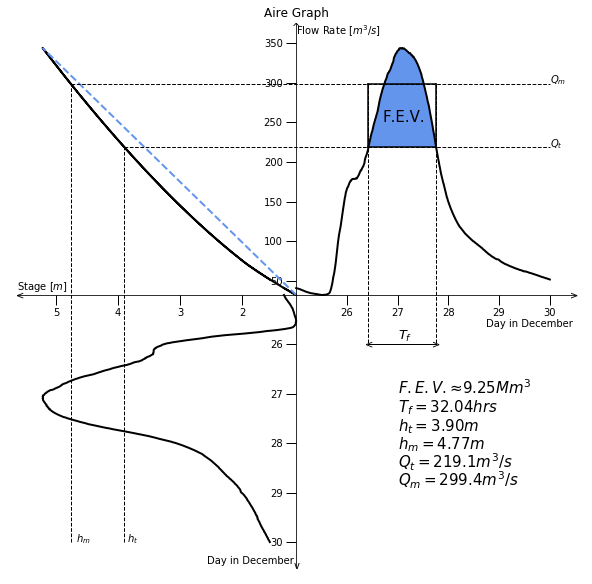
\includegraphics[scale=0.55]{Aire-Quadrant_Graph.png}}
\caption{Flow rate and river height data for the River Aire at the Armely gauging station in Leeds: a) river height ($\overline{h}$[m]) \cite{Aire} and catchment rainfall [mm] data \cite{NRFA} for a year starting from May 2015 (note, catchment rainfall data was not available for 2016) and b) quadrant plot for the 2015 Boxing Day floods of the River Aire. The top-left quadrant displays the rating curve (using data provided by Table 1) alongside its linear approximation (the blue dashed line), whilst the top-right and bottom-left quadrants display the river height ($\overline{h}$[m]) and flow rate ($Q$ [m$^3$/s]), respectively, during the floods. FEV is then the blue area below the flow rate curve (a function of $\overline{h}$, $Q(\overline{h})$, obtained from the rating curve) and above the flow rate corresponding to a given threshold height, $Q_T =Q(h_T)$. $\overline{h}=\overline{h}(t)$, where t is the number of days after the 25\textsuperscript{th} of December 2015, meaning $Q(\overline{h})=Q(t)$. Equation 2.1\textit{a} is applied to provide $V_e \approx V_{e_1}$= 9.34Mm$^3$, the blue shaded area. The emboldened rectangle approximates the FEV using equation 2.1\textit{c} so that $V_{e_2}= (Q_m -Q_T )\cdot T_f \approx V_{e_1}$= 9.34Mm$^3$, thereby providing an approximation of $Q_m$ given fixed $Q_T$=219.1m$^3$/s and calculated $T_f$=32 hours. Rearranging the rating curve equation 2.1 will provide an evaluation of $h_m$=4.77m from $Q_m$.}
\end{figure}

\begin{table}[H]
\centering
\begin{tabular}{l|l|l|l|l|l}
$k$ & $h_{k-1}$ [m] & $h_k$ [m] & $c_k$ [m$^{3-b_k}$/s] & $b_k$ [-] & $a_k$ [m]\\
\hline
1 & 0.2 & 0.685 & 30.69 & 1.115 & 0.156 \\
2 & 0.685 & 1.917 & 27.884 & 1.462 & 0.028 \\
3 & 1.917 & 4.17 & 30.127 & 1.502 & 0.153 \\
\end{tabular}
\caption{The coefficients $a_k$, $b_k$ and $c_k$ and their corresponding upper ($h_k$) and lower ($h_{k-1}$) bounds on $\overline{h}$ \cite{Aire} applied in the calculation of the rating curve, using equation 2.1, at the Armley gauging station on the River Aire.}
\end{table}

\subsubsection{Past and planned mitigation projects in Leeds}
\begin{figure}[H]
\centering
\subfloat[]{\includegraphics[scale=0.37]{Square-Lake1.png}}
\subfloat[]{\includegraphics[scale=0.37]{Square-Lake2.png}}
\hfill
\subfloat[]{\includegraphics[scale=0.37]{Square-Lake3.png}}
\subfloat[]{\includegraphics[scale=0.37]{Square-Lake4.png}}
\caption{}
\end{figure}

\subsection{The River Calder}

\begin{figure}[H]
\centering
\sidesubfloat[]{\includegraphics[scale=0.55]{Calder-Rainfall_Graph.png}}
\hfill
\sidesubfloat[]{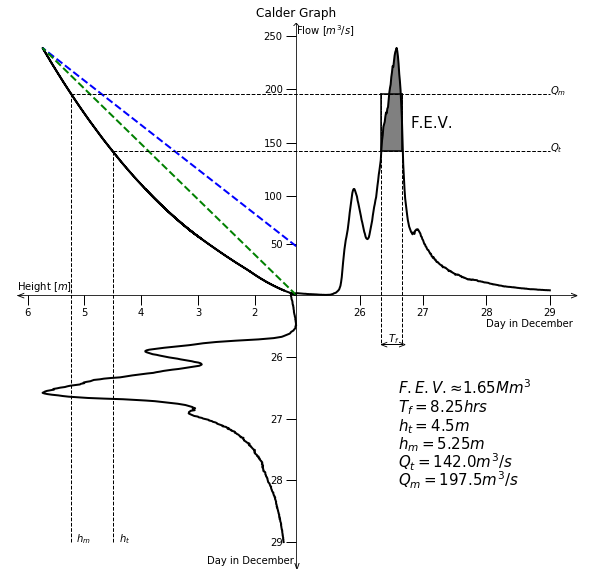
\includegraphics[scale=0.55]{Calder-Quadrant_Graph.png}}
\caption{Flow rate and river height data for the River Calder at the Mytholmroyd gauging station: a) river height ($\overline{h}$[m]) \cite{Calder-Don} and catchment rainfall [mm] data \cite{NRFA} for a year starting from May 2015 (note, catchment rainfall data was not available for 2016) and b) quadrant plot for the 2015 Boxing Day floods of the River Calder (\textit{cf.} Figure 1 b)).}
\end{figure}

\begin{table}[H]
\centering
\begin{tabular}{l|l|l|l|l|l}
$k$ & $h_{k-1}$ [m] & $h_k$ [m] & $c_k$ [m$^{3-b_k}$/s] & $b_k$ [-] & $a_k$ [m]\\
\hline
1 & 0 & 2.107 & 8.459 & 2.239 & 0.342 \\
2 & 2.107 & 3.088 & 21.5 & 1.37 & 0.826 \\
3 & 3.088 & 5.8 & 2.086 & 2.515 & -0.856 \\
\end{tabular}
\caption{The coefficients $a_k$, $b_k$ and $c_k$ and their corresponding upper ($h_k$) and lower ($h_{k-1}$) bounds on $\overline{h}$ \cite{Calder-Don} applied in the calculation of the rating curve, using equation 2.1, at the Mythomroyd gauging station on the River Calder.}
\end{table}

\subsubsection{Past and planned mitigation projects in Calderdale}

\section{Verification: The June 2007 flood of the River Don}
\begin{figure}[H]
\centering
\sidesubfloat[]{\includegraphics[scale=0.55]{Don-Rainfall_Graph.png}}
\hfill
\sidesubfloat[]{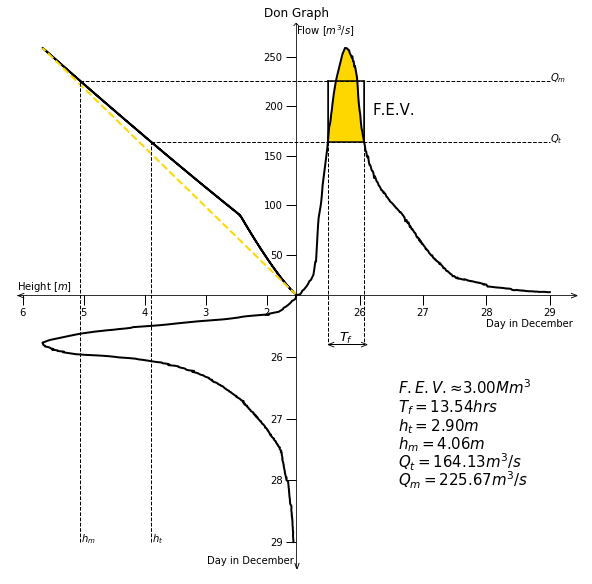
\includegraphics[scale=0.55]{Don-Quadrant_Graph.png}}
\caption{Flow rate and river height data for the River Don at the Sheffield Hadfields: a) river height ($\overline{h}$[m]) \cite{Calder-Don} and catchment rainfall [mm] data \cite{NRFA} for a year starting from January 2007 and b) quadrant plot for the June 2007 floods of the River Don (\textit{cf.} Figure 1 b)), where the time values in this case give the number of days after the 25\textsuperscript{th} of June 2007.}
\end{figure}

\begin{table}[H]
\centering
\begin{tabular}{l|l|l|l|l|l}
$k$ & $h_{k-1}$ [m] & $h_k$ [m] & $c_k$ [m$^{3-b_k}$/s] & $b_k$ [-] & $a_k$ [m]\\
\hline
1 & 0 & 0.52 & 78.4407 & 1.7742 & 0.223 \\
2 & 0.52 & 0.931 & 77.2829 & 1.3803 & 0.3077 \\
3 & 0.931 & 1.436 & 79.5956 & 1.2967 & 0.34 \\
4 & 1.436 & 3.58 & 41.3367 & 1.1066 & -0.5767 \\
\end{tabular}
\caption{The coefficients $a_k$, $b_k$ and $c_k$ and their corresponding upper ($h_k$) and lower ($h_{k-1}$) bounds on $\overline{h}$ \cite{Calder-Don} applied in the calculation of the rating curve, using equation 2.1, at the Sheffield Hadfields gauging station on the River Don.}
\end{table}

\subsection{Past and planned mitigation projects in Sheffield}

\section{Analysis: the November 2012 flood of the River Avon in Warwickshire}
\begin{figure}[H]
\centering
\subfloat{\includegraphics[scale=0.2]{Stratford-Flooding-Plaque.png}}
\subfloat{\includegraphics[scale=0.4]{Stratford-Flooded.jpg}}
\hfill
\subfloat{\includegraphics[scale=0.229]{Warwick-Castle.png}}
\subfloat{\includegraphics[scale=0.203]{Warwick-Castle-Flooded.png}}
\caption{Flooding in Stratford-upon-Avon and Warwick: the top left photo is of a plaque in Stratford-upon-Avon displaying historic flood height highs{;} it was erected before the 2012 flooding event \cite{plaque}. The top right is a photo of Bancfrotft in Stratford-upon-Avon during a flood \cite{strat-flood}. The bottom two photos are of the famous Warwick Castle, the left \cite{castle} unflooded and the right \cite{warwick-flooding} during a flood. The gauging stations in both Warwick and Stratford-upon-Avon are very slightly upstream from the Castle and Bancroft respectively meaning it is these areas of flooding that will be analysed.}
\end{figure}

Warwickshire has a long history of flooding as the large amount of agricultural land, which is relatively impervious, within the county makes it particularly vulnerable to surface water flooding whilst the large number of rivers, the two biggest being the River's Avon and Leam, make fluvial flooding a threat. Numerous flooding events in recent history confirm the risk that Warwickshire faces from floods. These include: January 1992, Easter 1998, August 1999, June 2005, June/July 2007, December 2008, November 2012, July 2014, December 2015 and August 2016 \cite{war2}. In fact, \textit{``around one in seven commercial properties and one in ten residential properties are at risk from flooding from rivers or surface water''} \cite{war1} in Warwickshire and that statistically \textit{``the fear of flooding is greater than the fear of crime in large areas of the county''} \cite{war1}. 

\subsection{The flood in Stratford-upon-Avon}
\begin{figure}[ht!]
\centering
\sidesubfloat[]{\includegraphics[scale=0.55]{Stratford-Rainfall_Graph.png}}
\hfill
\sidesubfloat[]{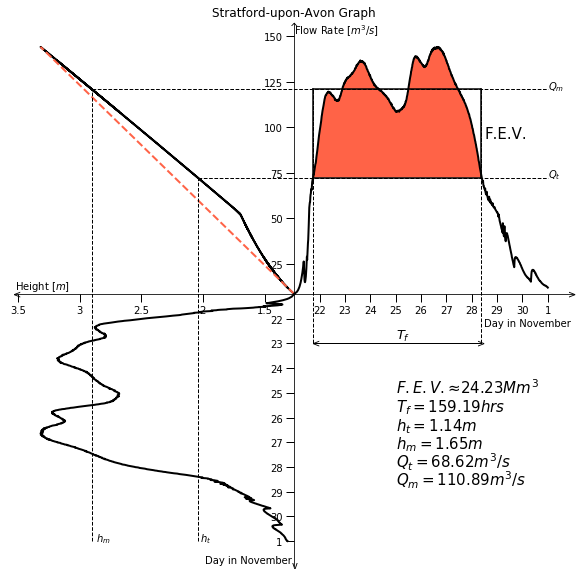
\includegraphics[scale=0.55]{Stratford-Quadrant_Graph.png}}
\caption{Flow rate and river height for the River Avon at the Cox's Yard gauging station in Stratford-upon-Avon: a) river height ($\overline{h}$[m]) \cite{EA} and catchment rainfall [mm] data \cite{NRFA} for the months of November and December 2012 (note, catchment rainfall data was not available for this gauging station so data was instead obtained for the next nearest geographical station, Alscot Park on the River Stour) and b) quadrant plot for the November 2012 floods of the River Avon at Stratford-upon-Avon (\textit{cf.} Figure 1 b)), where the time values in this case are the number of days from the 21\textsuperscript{st} of November 2012.}
\end{figure}

The local knowledge of the author about the plaque in Figure \textbf{insert} raised Stratford-upon-Avon, situated on the banks of the River Avon (an eastern tributary of the longest river in Britain, the River Severn \cite{britannica}), as a location of interest within Warwickshire that has a history of flooding. Although there have been many instances of flooding in Stratford-upon-Avon in recent years, River levels UK \cite{recent-high} states that the most recent high achieved by the River Avon at the Stratford-upon-Avon gauging station was during the November/December 2012 floods, reaching a river level of 1.89m at 15:30 on monday the 26\textsuperscript{the} of November. The government run flood information service \cite{ht} states that property flooding is possible in Stratford-upon-Avon once the River Avon has reached a height of 1.7m, and so this is the threshold height $h_T$ that will be used to calculated the FEV of the November 2012 floods. It should be noted that personal correspondance with the Environment Agency \cite{EA} suggested a threshold height of 1.2m but as the flood information surface states that low lying land may be flooded once the River Avon has reached 1.2m, the threshold height corresponding to a more significant flood of property is taken. The chosen threshold height of $h_T$= 1.7m yields
\begin{equation}\tag{5.1\textit{a}}
V_{e_1}(h_T=\text{1.7m})\approx 1.83\text{Mm$^3$},
\end{equation}
where $V_{e_1}(h_T=\text{1.7m})$ is found by applying equation 2.1\textit{b}. Thus, the less acurate approximation to $V_e$, $V_{e_3}(h_T=\text{1.7m})\approx 1.45\text{Mm$^3$}$ given by equation 2.1\textit{e} where the $Q_{max}$= 131.03m$^3$/s and $h_{max}$= 1.89m, is roughly 79\% of $V_{e_1}$. This is actually a relatively accurate approximation{;} the same approximation using equation 2.1\textit{e} for the FEV of the River Aire flood in 2015 performed in \S \textbf{insert} is just 65\% of the best approximation $V_{e_1}$. The river levels for the River Avon in Stratford-upon-Avon for November and December 2012 shown in Figure \textbf{insert} suggest another spike in the height of the river towards the end of December. The FEV for this flood has been calculated and found to be minimal in comparison to the FEV of the flood event in November. 

\begin{table}[ht!]
\begin{tabular}{l|l|l|l|l|l}
$k$ & $h_{k-1}$ [m] & $h_k$ [m] & $c_k$ [m$^{3-b_k}$/s] & $b_k$ [-] & $a_k$ [m]\\
\hline
1 & 0.136 & 0.938 & 158.04 & 2.85438 & 0.262919 \\
2 & 0.938 & 1.427 & 87.0362 & 0.962129 & 0.358741 \\
\end{tabular}
\caption{The coefficients $a_k$, $b_k$ and $c_k$ and their corresponding upper ($h_k$) and lower ($h_{k-1}$) bounds on $\overline{h}$ \cite{EA} applied in the calculation of the rating curve, using equation 2.1, at the Cox's Yard gauging station on the River Avon. This rating curve has then been used in the calculation of the FEV in Figure \textbf{insert}}
\end{table}

\begin{figure}[ht!]
\centering
\subfloat[]{\includegraphics[scale=0.55]{Stratford-FEV_ht_Graph.png}}
\hfill
\subfloat[]{\includegraphics[scale=0.56]{Stratford-Square_Lake_Graph.png}}
\subfloat[]{\includegraphics[scale=0.4]{Stratford-Adding_FEV_Graph.png}}
\caption{Stratford-upon-Avon square lake graphs for the November 2012 flood: a) is a visual aid demonstrating the relationship between a chosen $h_T$ and both its corresponding FEV (the red line with crosses) and square lake side length (the light blue line with circles) where b) demonstrates what is meant by square lake side length, the side length of our calculated FEV's (1.83Mm$^3$) 2m deep square lake being 956.56m. c) shows how the calculated FEV (\textit{cf.} Figure 1 b)) for the seperated peaks (the middle peak corresponds to the green line with triangles, the right peak to the blue line with circles and the leftmost peak, which then disapears above $h_T$ = 1.6m, to the black square) of $Q(t)$ above $Q_T$ (as seen in Figure 4 b)) is then added together to approximate the total FEV (the red line with crosses).}
\end{figure}

The FEV of 1.83Mm$^3$ can be handily represented by the capacity of a square lake of depth 2m with side-length 956.56m, as seen in Figure \textbf{insert}. The speculative nature of estimating $h_T$ means that the FEV of a flood can vary wildly depending on the chosen $h_T$. The relationship between possible threshold heights and the estimate of the FEV that they result in alongside their equivalent square lake of depth 2m side-length can be seen in Figure \textbf{insert}. The splitting of the flow rate into two peaks above the threshold flow rate $Q_T$ means the River actually floods twice in a short space of time in November 2012. The FEV of each peak must then be added to provide a value for the total FEV discharged during the floods of November 2012{;} Figure \textbf{insert} gives the FEV of each peak at a certain threshold height alongside the total FEV summing them provides. Although the mean flow rate of the River Avon once it has begun flooding at the Cox's Yard gauing station in Stratford-upon-Avon, $Q_m$= 123.26m$^3$/s, is much smaller than the \textbf{may have to delete if not reviewing calder flood} than the mean flow rate of the River Calder once it bagan flooding in December 2015, 197.50m$^3$/s \textit{cf.} Figure \textbf{insert}, the fact that the Stratford-upon-Avon flood lasted just under eight times as long makes the FEV produced by both of the floods comparable. 

\subsubsection{Verification: Stratford-upon-Avon FEV of November 2012}

\subsection{The flood in Warwick}
\begin{figure}[ht!]
\centering
\sidesubfloat[]{\includegraphics[scale=0.55]{Warwick-Rainfall_Graph.png}}
\hfill
\sidesubfloat[]{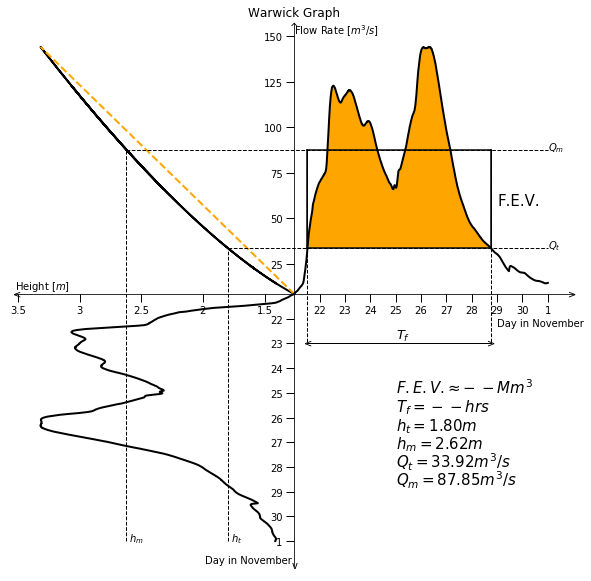
\includegraphics[scale=0.55]{Warwick-Quadrant_Graph.png}}
\caption{Flow rate and river height for the River Avon at the Warwick gauging station: a) river height ($\overline{h}$[m]) \cite{EA} and catchment rainfall [mm] data \cite{NRFA} for the months of November and December 2012. b) quadrant plot for the November 2012 floods of the River Avon at Warwick (\textit{cf.} Figure 1 b)), where the time values in this case are the number of days from the 21\textsuperscript{st} of November 2012.}
\end{figure}

\begin{table}[ht!]
\centering
\begin{tabular}{l|l|l|l|l|l}
$k$ & $h_{k-1}$ [m] & $h_k$ [m] & $c_k$ [m$^{3-b_k}$/s] & $b_k$ [-] & $a_k$ [m]\\
\hline
1 & 0.960 & 3.000 & 40.6178 & 1.44854 & 0.917837 \\
\end{tabular}
\caption{The coefficients $a_k$, $b_k$ and $c_k$ and their corresponding upper ($h_k$) and lower ($h_{k-1}$) bounds on $\overline{h}$ \cite{EA} applied in the calculation of the rating curve, using equation 2.1, at the Warwick gauging station on the River Avon.}
\end{table}

\begin{figure}[ht!]
\centering
\subfloat[]{\includegraphics[scale=0.55]{Warwick-FEV_ht_Graph.png}}
\hfill
\subfloat[]{\includegraphics[scale=0.6]{Warwick-Square_Lake_Graph.png}}
\subfloat[]{\includegraphics[scale=0.4]{Warwick-Adding_FEV_Graph.png}}
\caption{Warwick square lake graphs for the November 2012 flood: a) is a visual aid demonstrating the relationship between a chosen $h_T$ and both its corresponding FEV (the orange line with crosses) and square lake side length (the light blue line with circles) where b) demonstrates what is meant by square lake side length, the side length of our calculated FEV's (0.74Mm$^3$) 2m deep square lake being 908.28m. c) gives the individual FEV of seperated peaks when they occur {;}the leftmost peak corresponds to the black line with squares, the right peak to the blue line with circles and the middle peak, when it does exist, to the green triangles (\textit{cf.} Figure 6 c)). The total FEV is given by the orange line with crosses.}
\end{figure}

\noindent Having analysed the November 2012 flood in Stratford-upon-Avon, it would be useful to next investigate the same flood at the next gauging station upstream from Stratford-upon-Avon in order to determine where the best placement is for flood mitigation structures along the River Avon. That gauging station is the Warwick gauging station. The locations of the gauging stations in Stratford-upon-Avon and Warwick are given in Figure \textbf{insert} alongside an overview of the route of the River Avon between them. The flood information does not provide a river level at which property may be flooded in Warwick, the method of approximating $h_T$ used for Stratford-upon-Avon, but the Environment Agency estimates that the flooding of low lying land may occur above a level of 2.3m \cite{EA}. Thus, a rough estimate for the threshold height can be found by noticing that the level at which property may flood is roughly 40\% higher than the level at which low lying may flood in Stratford-upon-Avon. Thus $h_T$= 3.2m, 40\% higher than 2.3m, is the very rough threshold height used in the caculation of the FEV produced in Warwick during the November 2012 floods.

This threshold height yields an FEV of
\begin{equation}\tag{5.2\textit{a}}
V_{e_1}(h_T=\text{3.2m})\approx 0.45\text{Mm$^3$},
\end{equation}
using equation 2.1\textit{b}. The crudest approximation to $V_e$, $V_{e_3}(h_T=\text{3.2m})\approx 0.23\text{Mm$^3$}$ given by equation 2.1\textit{e} where the $Q_{max}$= 144.38m$^3$/s and $h_{max}$= 3.32m, is roughly 51\% of $V_{e_1}$ making $V_{e_3}$ a very poor approximation of $V_e$. An FEV of 0.45Mm$^3$ is the equivalent volume of a square lake of depth 2m with side-lengths 608.28m, as seen in Figure \textbf{insert}. The difference in the FEV's for Warwick and Straford-upon-Avon is expected, the River Avon should collect more surface water run-off, rain water and/or ground water as it flows from Warwick to Stratford-upon-Avon. However, the very large discrepancy in FEV may suggest that the approximate threshold height of 3.2m is too large. Figure \textbf{insert} shows the FEV of the Warwick flood given different values of $h_T$ and may imply that $h_T$ should be chosen to be in the range of 3m to 3.1m, which should result in an FEV of between 1.76Mm$^3$, and 0.99Mm$^3$.

\section{Main results: flood-mitigation cost efficacy assessment using FEV}
\subsection{Past and planned mitigation projects upstream of Stratford-upon-Avon}
\begin{figure}[ht!]
\begin{center}
\subfloat{\includegraphics[scale=0.5]{Stratford-Warwick_Risk.png}}
\caption{Flood-risk map for the stretch of the River Avon in between Warwick and Stratford-upon-Avon \cite{flood-risk}. The location of the gauging stations in Warwick and Stratford-upon-Avon are given by the orange and red markers repectively. St. John's brook is denoted by the green marker and the Racecourse brook by the yellow marker{;} each of which could potentially provide extra flood water storage.}
\end{center}
\end{figure}

Warwickshire County Council in association with the Environment Agency and Severn Trent Water have produced a local flood risk management strategy \cite{war1} that approaches that task of managing flooding from two angles, non-structural (aimed at mitigating the affects of a flood once it has begun as well as the general public's preparedness for a flood) and structural flood mitigation (aimed at preventing, or reducing the volume of, a flood). One example of non-structural flood mitigation being explored by the council is the introduction of a comprehensive sandbag protocol so that the public has quick and plentiful access to sandbags in the event of a flood. 

However, in order to perform a cost effictiveness assessment using FEV of different methods of flood mitigation, the volume the relevant mitigation policy reduces the FEV by must be quantifiable and as such the assessment in this report will be focussed solely on structural flood mitigation. There are two structural flood mitigation projects mentioned in the preperatory pack sent out to the English Severn and Wye regional flood coastal committee ahead of their meeting on tuesday the 8\textsuperscript{th} of January 2019 \cite{brook} which are the planned building of two brooks, the St John's brook in Warwick and the Racecourse brook in Stratford-upon-Avon. Other structural flood mitigation projects that have already been undertaken was the building of portable flood barriers owned by the Environment Agency that can be deployed ahead of a predicted flood, the installation of three pumps at the Stanford-on-Avon reservoir to enable the drawing down of the reservoir before predicted heavy rainfall  as well as improvements to the storage capacity of the spillway of the reservoir.

St John's brook in Warwick (The green marker in Figure \textbf{fill in}) is expected to be built less than 50 metres upstream of the river level gauging station in Warwick (the orange marker in Figure \textbf{fill in}) and is expected to be provide 32000m$^3$ of flood water storage potential at a cost of \pounds1.45M whilst the Racecourse brook in Stratford-upon-Avon (represented by the yellow marker in Figure \textbf{fill in}) will give around 16000m$^3$ of storage for \pounds720000 \cite{brook}. Both brooks therefore provide 48000m$^3$ (equivalent to 2.62\% of the November 2012 flood in Stratford-upon-Avon) of extra flood water storage. Taking the annual maintenance costs to be \pounds600 \cite{cost4} for both brooks, the price for installation and maintenance of the brooks over 50 years is approximately \pounds2.2M meaning that the price of the two projects per percentage of FEV mitigated is \pounds0.84M.

The third structural flood mitigation project is the manufacturing of 40km of temporary portable flood barriers by the Environment Agency for use in numerous locations including Stratford-upon-Avon \cite{lentemp}. This project has recently been completed and a flooding scenario simulation involving the barrier has been undertaken in the centre of Stratford-upon-Avon \cite{strat-flood}. The cost per metre of constructing the barrier has been estimated to be between \pounds5 and \pounds10, meaning the cost of constructing 40km is in the range of \pounds[0.2, 0.4]M. The cost of the full 40km is included as it needs to be this length so that it can be used in numerous locations during a flood as if Stratford-upon-Avon is flooded then it is likely other locations near to Stratford-upon-Avon will be flooded and thus need the barriers too. The cost per deployment of these barriers is estimated to be in the range of \pounds[1000, 20000] \cite{temp}, and this along with the knowledge that the Avon has flooded 10 times (as mention in \S\textbf{fill in} since January of 1992, the cumulative costs of deployment over 50 years can be approximated as \pounds[19000, 380000]. Assuming an average annual maintenance cost of \pounds5 per m \cite{cost1}, giving a 50 year maintenance cost of 40km of barrier of \pounds10M, the cost of building, running and maintaining the temporary flood barriers for 50 years is \pounds[10.22, 10.38]M. The temporary nature of the barriers make it difficult to quantify the percentage of FEV mitigated because if the barrier is properly and punctually in place before the flood being then 100\% of the FEV is mitigated. If, however, the barrier is not put in place in time then 0\% of the FEV will be mitigated. Thus, the cost per percentage of FEV mitigated could potentially be \pounds[0.102, 0.104]M if the barrier is in place every time the river floods{;} on the other hand, the project cost of \pounds[10.22, 10.38]M may not mitigate the flood at all if it is never in place when the river floods and is therefore a wasted expense. More detailed assessment on the probability of the barrier being in place is therefore needed before any conclusions may be drawn.

Upstream of Warwick there is a drinking water reservoir in Stanford-on-Avon, known as the Stanford reservoir, that has a maximum capacity of 500M gallons, equivalent to 2.27Mm$^3$ \cite{volume}. In 2017, the installation of what the Environment Agency classifies as `large' pumps, capable of pumping 415 litres of water a second out of the reservoir \cite{pump}, has allowed for the possibility of reducing the volume of the reservoir by 10\% ahead of predicted heavy rainfall so as to provide an additional 0.227m$^3$ of flood water storage, thereby mitigating downstream flooding in such places as Warwick and Stratford-upon-Avon by this volume. The estimated capital cost of the installation of a large pump is \pounds0.41M alongside annual maintenance, annual running and annualised periodic refurbishment costs of \pounds8000, \pounds5000 and \pounds13000 respectively \cite{cost2}. Therefore the cost over 50 years of three large pumps is \pounds5.13M and as 0.227m$^3$ constitutes 12.4\% of the FEV in Stratford-upon-Avon, this is equivalent to \pounds0.41M per 1\% of the FEV mitigated.

As part of the project that involved the installation of the three pumps in the Stanford reservoir, an extension of the spillway of the reservoir was conducted. This involved widening the 6m deep and 1.73km long spillway by 5.4m to a new width of 11.5m \cite{spillway}, providing an extra 56052m$^3$ of flood water storage. The widening of the spillway itself should not necessitate the need for any more maintenance besided that which the unwidened spillway required anyway. The budget of the project, including the installation of the pumps, is given to be \pounds2.4M \cite{spillway} meaning the estimated cost of the spillway modifications can be estimated as the overall cost of the project minus the capital cost of installing three large pumps, as provided above. This estimated cost is therefore \pounds1.17M and as 56052m$^3$ is 3.06\% of the FEV of the November 2012 flood in Stratford-upon-Avon, the esimated cost of widening the spillway per percentage of the FEV mitigated is \pounds0.38M.

Having performed a cost efficacy assessment of structural flood mitigation tactics in and around Warwickshire and how they could affect flooding in Stratford-upon-Avon, various hypothetical scenarios will now be similarly assessed and then compared with the nonspeculative methods discussed above.

\subsection{Sustainable urban drainage systems (SuDS)}
Sustainable urban drainage systems (or SuDS) encompasses flood mitigation techniques aimed at reducing the detrimental effects of urbanisation has on surface water run off rates, which can cause both surface water and flooding \cite{suds}. Types of SuDS include green roofs and permeable paving and the potenetial effect of installing 50000m$^2$, comprising an area sufficiently smaller than the area comprised of the Stratford-upon-Avon town limits, of each of these kinds of SuDS within Stratford-upon-Avon will be specifically explored. The estimated cost per m$^2$ of installing green roofs and permeable pavements is \pounds90 and \pounds40 alongside 50 year maintenance costs of \pounds313 and \pounds20 respectively \cite{cost3}. Hence, the combined cost over 50 years of 50000m$^2$ of green roofs and 50000m$^2$ is approximately \pounds22.17M. Models of both green roofs and permeable pavements and their affects on the volume of a flood have shown that about 0.116m$^3$ and 0.138m$^3$ of the flood is mitigated per m$^2$ of green roofing and permeable paving respectively \cite{suds}. Therefore, the combined effects of 50000m$^3$ of each of these methods could mitigate a flood by as much as 12700m$^3$, comprising 0.69\% of the FEV. The cost per 1\% of FEV is then found to be \pounds32.13M, an extremely large value. The apparent exceedingly poor cost effectiveness of SuDS in relation to the purpose of mitigating a flood may explain why Warwickshire County Council have decided to make it a requirement for any new properties built to have enough SuDS to mitigate their negative effect on surface water flooding \cite{war2}{;} as opposed to simply buying and installing new SuDS themselves.

\subsection{Natural flood management}
The term natural flood management (NFM) is an umbrella term describing the use of natural processes in reducing the risk and subsequent impact of flooding \cite{NFM}. NFM can be broadly divided into 4 main subcategories which are the management of: the river and the flood plain itself, the causes of run off, woodland within the catchment area of the river and, finally, the coast \cite{nfm}. Coastal flooding is not within the remit of this report and as some examples of run-off management were explored in \S \textbf{insert}, the next two flood mitigation ideas will focus on the first two listed subcategories of NFM.

\subsubsection{Flow-attenuation features}
Flow-attenuation features are designed to reduce the flow rate of a river, thereby reducing the FEV produced by a river over the same time interval, with the aid of natural processes. The flood management scheme in Blackbrook, St Helens, has comprised of the construction of four engineered log dams at a cost of \pounds2000 \cite{nfm}. These types of leaky dams are designed to allow the passage of water when it is moving at a low flow rate but to then reduce the flow of the river once the flow rate increases and the combination of the four dams in Blackbrook is expected to mitigate the FEV by 2500m$^3$ \cite{blackbrook}. Scaling up this project by a factor of 20 would then involve the building of eighty of these leaky dams spread evenly along the River Avon upstream of Stratford-upon-Avon and would constitute a reduction in the FEV of 50000m$^3$. The natural nature of a leaky dam makes the life span of one limited and so, assuming a life span of 25 years, the base cost of building the eighty dams, \pounds40000, would need to be doubled over a 50 year period. Regular maintenance would also have to performed throughout the 50 years and so, by assuming the need for one permanently employed maintenance worker with an annual salary of \pounds50000, the total 50 year cost of eighty engineered log dams can be expected to be in the region of \pounds2.58M. As 50000m$^3$ is the equivalent of 2.73\% of the FEV, the approximate cost of installing eighty log dams is \pounds0.95M.

\subsubsection{Tree planting}
The planting of new forestation reduces the impact of flooding by effectively `drinking' rainwater from the ground thereby extending the length of time it takes ground to become water logged at which point any excess rain fall would run into the river, contributing to fluvial flooding. There is a flood mitigation scheme for the River Torne in Doncaster that has involved the creation of 46.5 hectares (equivalent to 0.465km$^2$) of new catchment woodland which provided over 4000m$^3$ of extra flood storage capacity at a cost of \pounds130000 \cite{nfm}. The catchment area of the River Avon is 2308km$^2$ \cite{britannica} and one hypothetical flood mititgation measure could be the transformation of 3\% of this area into woodland. This would be equivalent of the creation of 69.24km$^2$ of new forest or reproducing the River Torne scheme 148.9 times over. This scenario would then have a base cost of \pounds19.36M which would provide additional flood storage of 596000m$^3$, or 32.57\%. An estimation of the maintenance cost per km$^2$ of new woodland is \pounds864 \cite{cost1}, giving the 50 year cost of maintaining 69.24km$^2$ to be \pounds2.99M. Thus, the cost per percentage of the FEV mitigated is estimated to be \pounds0.69M.

\subsection{Giving room to the river}
\subsubsection{Theory}
\begin{figure}[ht!]
\begin{center}
\sidesubfloat[]{\includegraphics[scale=0.4]{GRR-1.png}}
\hfill
\sidesubfloat[]{\includegraphics[scale=0.555]{GRR-Graph.png}}
\caption{Giving-room-to-the-river: a) is a heavily simplified transverse profile of the River Avon if it were to be widened by 3.5m at a height of 0.5m on one bank where its width before the process is 41.5m and its threshold height remains as it was before, 1.7m \cite{maps}. The gradient of the new slope (1/b) is approximately the same as before the process {;} b) is a zoom in of the top left quadrant of Figure 6. It is a plot of the flow rate $Q(\overline{h})$ against t, \textit{cf.} Figure 6 b). The threshold level $h_T$ does not change as part of the GRR process but the relationship between $\overline{h}$ and Q, the rating curve, does. The two threshold flow rates on the graph, $Q_{T}$ and $Q_{T_{GRR}}$, correspond to the river before it is widened and after respectively. Thus, the FEV mitigated by the GRR process can be quantified as the difference of the FEV's given by the two different threshold flow rates, $V_{e}-V_{e_{GRR}}$ = 0.99Mm$^3$/s, which is equivalent to $\approx 54.10\%$ of the FEV before GRR. $V_{e_{GRR}}$ is the equivalent of the shaded red region on the graph and $V_{e}$ is the FEV calculated in Figure \textbf{insert}.}
\end{center}
\end{figure}

\noindent The option explored here involves the widening of the river bed along the stretch of the River Avon that flows through Stratford-upon-Avon, a process that is also known as giving-room-to-the-river (GRR). Figure \textbf{insert} gives an overview of the chosen location as well as the approximate length of the stretch of river that is proposed to be widened, 1.72km. In the 1800's, an engineer, R. Manning, discovered a formula that could be applied to find the flow rate $Q$ of a stretch of fluid in an open channel 
\begin{equation}\tag{6.4.1\textit{a}}
Q=\frac{k}{n}AR^{2/3}S^{1/2},
\end{equation}
given a parameter $n$, the longitudinal slope of the river bed $S$, the hydraulic radius $R$ of the channel and the cross sectional area of the fluid in the channel $A$ \cite{manning}. As this report deal with quntites within the internation system of units, $k$=1 \cite{manning}. The hydraulic radius $R$ of the channel is defined as the cross sectional area $A$  divided by the wetted perimeter $P$ meaning equation 6.4.1\textit{a} may be re-written as
\begin{equation}\tag{6.4.1\textit{b}}
Q=\frac{\sqrt{S}}{n}\frac{A^{5/3}}{P^{2/3}}.
\end{equation}

If a river is proposed have one if its banks widened by length $w$ at a height of $h_b$ above the river bed, the cross sectional area of the river when it is at level $\overline{h}$ above $h_b$ will be increased by $w(\overline{h}-h_b)$. This is equivalent to the area of the dashed parellogram in Figure \textbf{insert} with width $w=$ 3.5m and height $\overline{h}-h_b$ where $h_b=$ 0.5m. Similarly, the wetted perimeter of the river will increase by $w+(\overline{h}-h_b)\sqrt{1+b^2}$, equivalent to the perimeter of the left hand side of the parallelogram in Figure \textbf{insert}. Thus, the change in flow rate $Q$ for a river widened along one bank by length $w$ at height $h_b$ above the river bed is
\begin{equation}\tag{6.4.1\textit{c}}
\Delta Q=\frac{\sqrt{S}}{n}\cdot\frac{(w(\overline{h}-h_b))^{5/3}}{(w+(\overline{h}-h_b)\sqrt{1+b^2})^{2/3}}.
\end{equation}
Thus, the total flow rate of a river $Q_{GRR}$ once it has undergone the giving-room-to-the-river procedure, will be given by adding the change in flow rate, $\Delta Q$, to the original flow rate $Q(\overline{h})$. In the case of the hypothetical widening of the River Avon in Stratford-upon-Avon, both banks are suggested to be widened not one{;} in which case $\Delta Q$ will double and
\begin{equation}\tag{6.4.1\textit{d}}
Q_{GRR}=Q(\overline{h})+2\Bigg[\frac{\sqrt{S}}{n}\cdot\frac{(w(\overline{h}-h_b))^{5/3}}{(w+(\overline{h}-h_b)\sqrt{1+b^2})^{2/3}}\Bigg].
\end{equation}

The proposal for this hypothetical situation is that the River Avon have both of its banks widened by $w=$ 3.5m at a height $h_b=$ 0.5m above the river bed. The Gauckler-Manning constant $n$ is dependant on numerous factors but most significantly the sinuosity and roughness of the channel the river flows through \cite{manning}. The River Avon can thus be expected to have a Gauckler-Manning constant of around 0.045, the typical value of $n$ for a winding channel with some vegetation and stones \cite{n}. The Encyclopedia Britannica \cite{britannica} sates that the length of the River Avon, 154km, corresponds to a fall of 150m. Therefore, the average longitudinal slope of the River Avon $S$ is 0.001. Choosing b to be 1.73 and using the values for $w$, $h_b$, $n$ and $S$ gives the threshold flow rate after the GRR process $Q_{T_{GRR}}$ to be
\begin{equation}\tag{6.4.1\textit{e}}
Q_{T_{GRR}}=Q_T+2\Bigg[\frac{\sqrt{0.001}}{0.045}\cdot\frac{(3.5(h_T-0.5))^{5/3}}{(3.5+(h_T-0.5)\sqrt{1+1.3^2})^{2/3}}\Bigg],
\end{equation}
where $Q_T$ and $h_T$ are as given in Figure \textbf{insert}. This is because although the channel the River Avon flows through is being widened, the height of the channel does not change meaning that neither will the height at which the River bursts its banks ($h_T$). Thus the threshold flow rate of the River Avon in Stratford-upon-Avon after the channel has been widened is $Q_{T_{GRR}}$= 120.37m$^3$/s, where $h_T$= 1.7m, which would then result in an FEV of 0.84Mm$^3$ (the red shaded area in Figure \textbf{insert}). The FEV has then been reduced by 0.99Mm$^3$, or 54.10\% of the FEV of the November 2012 floods in Stratford-upon-Avon.

\subsubsection{Cost efficacy assessment}
\begin{figure}[ht!]
\subfloat{\includegraphics[scale=0.4]{GRR-sat.png}}
\subfloat{\includegraphics[scale=0.483]{GRR-map.png}}
\caption{Satellite (left) and map (right) view \cite{maps} of the proposed stretch of the river to undertake giving-room-to-the-river, i.e. the stretch of river that flows through Stratford-upon-Avon that when flooded puts properties at risk. The right photo gives the approximate length of this stretch of the river as 1.72km.}
\end{figure}

\noindent The cost per metre of excavating a channel of depth 1.5m and width 20m is \pounds1510, assuming that a third of the of the material excavated is disposed of off-site \cite{cost1}. This constitutes a channel of cross sectional area 30m$^2$ whilst the River Avon channel in Stratford-upon-Avon is estimated to have average width 41.5m \cite{maps} with a depth of 1.7m, equivalent to $h_T$, resulting in a cross sectional area of 70.55m$^2$. The River Avon channel is thus approximately 2.35 times the size of the channel whose excavation costs \pounds1510 per metre meaning this cost can be scaled up to provide a rough estimate of the price for excavating the channel in Stratford-upon-Avon, \pounds3548.50 per metre. Figure \textbf{insert} gives that the channel through Stratford-upon-Avon is 1.72km long so the cost of giving-room-to-the-river for the entirety of this channel is \pounds6.10M. The banks of the River Avon are heavily cladded as it passes through Stratford-upon-Avon and the cost of replacing this heavy cladding onto the newly excavated channel would be \pounds1075 per metre per banking or \pounds3.70M per 1.72km of both banks. Similarly to the widening of the Stanford reservoir spill way in \S \textbf{insert}, the cost of maintaining the channel before and after it has undergone GRR should be the same meaning these costs will not be considered as part of the total cost. In \S \textbf{insert}, the percentage the FEV is reduced by was found to be 54.10\%. The cost of mitigating by this percentage has now been found to be \pounds9.80M which means the price per percentage of the FEV mitigated is \pounds0.18M.

\section{Summary and discussion}
\begin{figure}[ht!]
\subfloat[]{\includegraphics[scale=0.37]{Stratford-Square_Lake1.png}}
\subfloat[]{\includegraphics[scale=0.37]{Stratford-Square_Lake2.png}}
\hfill
\subfloat[]{\includegraphics[scale=0.37]{Stratford-Square_Lake3.png}}
\subfloat[]{\includegraphics[scale=0.37]{Stratford-Square_Lake4.png}}
\caption{}
\end{figure}

\begin{table}[ht!]
\centering
\begin{tabular}{l|l}
Flood mitigation measure & Cost per percentage of FEV mitigated [\pounds]\\
\hline
\textbf{Nonspeculative} & \\
The St. Johns and Racecourse brooks & 0.84M\\
Temporary flood barriers & 0.10M\\
Drawing down of the Stanford reservoir & 0.41M\\
Widening of the Stanford reservoir spillway & 0.38M\\
\textbf{Hypothetical} & \\
Green roofs and permeable paving& 32.13M\\
Flow-attenuation features & 0.95M\\
Tree planting & 0.69M\\
Giving-room-to-the-River & 0.18M\\
\end{tabular}
\caption{Table showing the cost, over 50 years, of mitigating the FEV of the November 2012 floods in Stratford-upon-Avon by 1\% by implementing each of the flood mitigation measure assessed in this report. The flood mitigation measures are splot into those that are nonspeculative, i.e. they have already been or are planning to be undertaken, and hypothetical scenarios.}
\end{table}

\subsection{Futher Reading}
The main source of information in regards to the flood-excess volume analysis used in this report was provided from the two articles \cite{Aire} and \cite{Calder-Don}, co-authored by the supervisors of this project, O. Bokhove and T. Kent. As such it would be beneficial to read these articles if there is a wish gain a broader understanding of the subject. Detailed information on the various methods of NFM is provided by the Environment Agency in \cite{nfm}, their study into working with natural processes. More information on what may happen in the future in regards to flood management nation wide is included \cite{foresight}, produced by the Flood and Coastal Defence project of the Foresight programme.

As part of this project the author, with the assistance of A. Feilden, S. Kennet, M. Saunders and J. Willis, has created two web pages, one giving information on the wider project as well as each individuals chosen rivers\footnote{The web page giving an over arching description of the project, and each team members individual work, can be found on GitHub at https://github.com/Rivers-Project-2018/Group-Project} and another  containing all the instruction nessecary to perform the same FEV analysis as in this report\footnote{The web page giving instructions on how to FEV analysis can be found on GitHub at https://github.com/Rivers-Project-2018/How-to-do-FEV-Analysis}. This includes an automated code which only needs the parameters of the rating curve and a chosen $h_T$ to produce a graph and provide an evaluation of the FEV, $Q_m$, $Q_T$, $h_m$ and $T_f$ as well as a three dimensional visualisation of the FEV's corresponding square lake of depth 2m. This code was written individually by the author with credit to A. Feliden for suggesting attaching an automated code for producing a representation of the 2m deep square lake. The code and the graphs it produces may be found in the Appendix. 

There are some limits to the automated nature of this code, such as the fact that if the curve $Q(\overline{h})$ is split into more than one peak above $Q_T$ then, although the FEV calculated will be accurate, $T_f$ and thereby $Q_m$ and $h_m$ will not. The code also will not work if the flood data being analysed does not cover an integer number of days. Therefore, if this project were to be continued, the fixing of these issues would be undertaken. Another web page\footnote{The web page containing the data sets, rating curve information and code used in this report can be found on GitHub at https://github.com/Rivers-Project-2018/Abbey-Chapman} created by the author includes all the data sets and rating curve information integral to the calculations of FEV in this report as well as the basic code for the included graphs.

\subsection{Acknowledgements}
The author would like to thank and acknowledge the Environment Agency in the West Midlands for contributing river height and flow rate data for the Warwick and Cox's Yard gauging stations, alongside each stations rating curve information, towards this report. This report contains public sector information licensed under the Open Government Licence v3.0.

\newpage
\section{References}
\begin{thebibliography}{}
\bibitem{foresight}
Flood and Coastal Defence Project of the Foresight programme. \textit{Foresight: Future Flooding}. [Online]. 2004. [Accessed 14 March 2019]. Available from: https://assets.publishing.service.gov.uk/

\bibitem{telegraph}
Burn-Callander, R. \textit{UK flooding: cost of damage to top £5bn but many homes and businesses underinsured}. [Online]. 2015. [Accessed 14 March 2019]. Available from: https://www.telegraph.co.uk/

\bibitem{yue}
Peters, H. \textit{Tattooed Faces and Stilt Houses: Who Were the Ancient Yue?}. [Online]. 1990. [Accessed 14 March 2019]. Available from: http://sino-platonic.org/

\bibitem{war2}
Warwickshire County Council. \textit{Surface Water Management Plan Methodology Report}. [Online]. 2015. [Accessed 14 March 2019]. Available from: https://apps.warwickshire.gov.uk/

\bibitem{war1}
Warwickshire County Council. \textit{Local Flood Risk Management Strategy}. [Online]. 2016. [Accessed 14 March 2019]. Available from: https://apps.warwickshire.gov.uk/

\bibitem{}
GaugeMap. \textit{Stratford (River Avon), Warwick (River Avon)}. [Online]. 2019. [Accessed 14 March 2019]. Available from: https://www.gaugemap.co.uk/

\bibitem{}
BBC News \textit{Warwickshire floods: Three swept away in car escape injury}. [Online]. 2012. [Accessed 14 March 2019]. Available from: https://www.bbc.co.uk/

\bibitem{castle}
Brown, E. \textit{Warwick Castle - River Avon, Warwick}. [Online]. 2016. [Accessed 14 March 2019]. Available from: https://www.flickr.com/

\bibitem{warwick-flooding}
Dimmer, S. \textit{Flood alerts issued for parts of Warwickshire}. [Online]. 2015. [Accessed 14 March 2019]. Available from: https://www.coventrytelegraph.net/

\bibitem{brook}
English Severn \& Wye. \textit{Regional Flood Coastal Committee: Tuesday 8 January 2019 agenda}. [Online]. 2019. [Accessed 14 March 2019]. Available from: https://assets.publishing.service.gov.uk/

\bibitem{recent-high}
River Levels. \textit{River Avon at Stratford}. [Online]. 2019. [Accessed 14 March 2019]. Available from: https://riverlevels.uk/

\bibitem{plaque}
Smith, C. \textit{Updated: River Avon remains on flood alert despite falling water levels}. [Online]. 2018. [Accessed 14 March 2019]. Available from: http://www.stratford-herald.com/

\bibitem{canal}
UK Waterways Guide. \textit{A brief history of the River Avon}. [Online]. 2019. [Accessed 14 March 2019]. Available from: https://www.ukwaterwaysguide.co.uk/

\bibitem{}
susdrain. \textit{Stroud Rural Suds, Stroud}. [Online]. 2018. [Accessed 14 March 2019]. Available from: https://www.susdrain.org/

\bibitem{}
Woodland Trust. \textit{Natural flood management guidance: Woody dams, deflectors and diverters}. [Online]. 2016. [Accessed 14 March 2019]. Available from: https://www.woodlandtrust.org.uk/

\bibitem{leaky-dams}
Rural Payments Agency and Natural England. \textit{RP33: Large leaky woody dams}. [Online]. 2017. [Accessed 14 March 2019]. Available from: https://www.gov.uk/

\bibitem{ht}
Flood information service. \textit{River level: River Avon at Stratford}. [Online]. 2019. [Accessed 14 March 2019]. Available from: https://flood-warning-information.service.gov.uk/

\bibitem{Aire}
Bokhove, O., Kelmanson, M. and Kent, T. \textit{On using flood-excess volume in flood mitigation, exemplified for the River Aire Boxing Day Flood of 2015}. [Online]. 2018. [Accessed 14 March 2019]. Available from: https://eartharxiv.org/

\bibitem{NRFA}
National River Flow Archive. \textit{NERC CEH, Warwick, Armely, Mytholmroyd, Sheffield Hadfields, Alscot Park}. [Online]. 2019. [Accessed 14 March 2019]. Available from: https://nrfa.ceh.ac.uk/

\bibitem{NFM}
Environment Agency. \textit{Natural flood management – part of the nation’s flood resilience}. [Online]. 2017. [Accessed 14 March 2019]. Available from: https://www.gov.uk/

\bibitem{suds}
Bayon, J., Charlesworth, S., Jato-Espino and Warwick, F. Rainfall–Runoff Simulations to Assess the Potential of SuDS for Mitigating Flooding in Highly Urbanized Catchments. \textit{International Journal of Environmental Research and Public Health}. 2016, \textbf{13}(1), 149.

\bibitem{flood-risk}
Environment Agency. \textit{Likelihood of flooding in this area}. [Online]. 2017. [Accessed 14 March 2019]. Available from: https://flood-map-for-planning.service.gov.uk/

\bibitem{Calder-Don}
Bokhove, O., Kelmanson, M. and Kent, T. \textit{On using flood-excess volume to assess natural flood management, exemplified for extreme 2007 and 2015 floods in Yorkshire}. [Online]. 2018. [Accessed 14 March 2019]. Available from: https://eartharxiv.org/

\bibitem{EA}
Weston, M. on behalf of the Environment Agency in the West Midlands. \textit{Email to Abbey Chapman}. 20 November, 2018.

\bibitem{strat-flood}
Lugg, B. \textit{New emergency flood barrier tested in Stratford}. [Online]. 2017. [Accessed 15 March 2019]. Available from: http://www.stratford-herald.com/

\bibitem{cost1}
Environment Agency. \textit{Cost estimation for channel management}. [Online]. 2015. [Accessed 14 March 2019]. Available from: http://evidence.environment-agency.gov.uk/

\bibitem{cost2}
Environment Agency. \textit{Cost estimation for control assets}. [Online]. 2015. [Accessed 15 March 2019]. Available from: http://evidence.environment-agency.gov.uk/

\bibitem{britannica}
The Editors of Encyclopedia Britannica. \textit{River Avon}. [Online]. 2017. [Accessed 15 March 2019]. Available from:  https://www.britannica.com/

\bibitem{trees}
Natural England. \textit{Countryside Stewardship Manual: Woodland Creation Grant}. [Online]. 2018. [Accessed 15 March 2019]. Available from: https://assets.publishing.service.gov.uk/

\bibitem{altitude}
Route Calculator. \textit{Altitude Stratford-upon-Avon, Warwick, UK}. [Online]. 2019. [Accessed 16 March 2019]. Available from: https://routecalculator.co.uk/

\bibitem{crow}
Doogal. \textit{Measuring distances}. [Online]. 2019. [Accessed 16 March 2019]. Available from: https://www.doogal.co.uk/

\bibitem{n}
FishXing. \textit{Manning's n Values}. [Online]. 2006. [Accessed 16 March 2019]. Available from: http://www.fsl.orst.edu/

\bibitem{manning}
Okiishi, T., Musnon, B. and Young, D. \textit{Fundamentals of Fluid Mechanics}. [Online]. . [Accessed 16 March 2019]. Available from: 

\bibitem{nfm}
Environment Agency. \textit{Working with Natural Processes - Evidence Directory}. [Online]. 2018. [Accessed 16 March 2019]. Available from: https://assets.publishing.service.gov.uk/

\bibitem{maps}
Google Maps. \textit{Google Maps}. [Online]. 2019. [Accessed 17 March 2019]. Available from: https://www.google.com/

\bibitem{volume}
Stanford Ringing Group. \textit{About Stanford Reservoir}. [Online]. 2001. [Accessed 17 March 2019]. Available from: http://stanfordrg.org.uk/

\bibitem{temp}
Shropshire Star. \textit{Protecting Shropshire from floods - this winter cost £45,000 keeping our homes dry}. [Online]. 2016. [Accessed 17 March 2019]. Available from: https://www.shropshirestar.com/

\bibitem{pump}
Water Active. \textit{Sykes provides overpump for Stanford reservoir spillway}. [Online]. 2017. [Accessed 17 March 2019]. Available from: http://www.wateractive.co.uk/

\bibitem{lentemp}
Environment Agency. \textit{Major flood defence exercise in Stratford}. [Online]. 2017. [Accessed 17 March 2019]. Available from: https://www.gov.uk/

\bibitem{spillway}
UK Water Projects Online. \textit{Stanford Reservoir Spillway Extension}. [Online]. 2018. [Accessed 17 March 2019]. Available from:

\bibitem{floodsource}
Environment Agency. \textit{Sources of flooding}. [Online]. 2013. [Accessed 17 March 2019]. Available from: https://webarchive.nationalarchives.gov.uk//floods/31652.aspx

\bibitem{cost3}
Environment Agency. \textit{Cost estimation for SuDS - summary of evidence}. [Online]. 2015. [Accessed 17 March 2019]. Available from: http://evidence.environment-agency.gov.uk/

\bibitem{cost4}
Environment Agency. \textit{Cost estimation for flood storage - summary of evidence}. [Online]. 2015. [Accessed 18 March 2019]. Available from: http://evidence.environment-agency.gov.uk/

\bibitem{blackbrook}
The Mersey Forest. \textit{New natural leaky dams installed in St Helens and Ellesmere Port}. [Online]. 2017. [Accessed 18 March 2019]. Available from: https://www.merseyforest.org.uk/

\bibitem{}
. \textit{}. [Online]. . [Accessed 16 March 2019]. Available from:
\end{thebibliography}


\newpage
\appendix
\section{Appendix}
{\bf The graph that the automated FEV code produces using the example of the 2015 Boxing Day flood of the River Aire at Armley as an example}\\
\begin{figure}[H]
\begin{center}
\subfloat{\includegraphics[scale=0.55]{Automated-Graph-Aire.png}}
\end{center}
\end{figure}

\noindent{\bf The automated FEV code written in the python coding language}\\
\begin{spacing}{1}\footnotesize{\lstinputlisting[language=Python]{Automated-Quadrant-Graph-Code.py}}
\end{spacing}

\vspace{1cm}
\noindent{\bf The python code used to produce Figure 1. a)}\\
\begin{spacing}{1}\footnotesize{\lstinputlisting[language=Python]{Aire-Rainfall_Graph.py}}
\end{spacing}


\end{document}
